\subsection{Challenge 2: Requirements Refinement}

When systems are decomposed into components, deriving the component requirements from the system requirements is a challenging task. While formal tools help to automatically verify the sufficiency of component requirements to guarantee the system level requirement, deriving and formalizing those component requirements has been a manual activity. However, it is possible to derive and formalize a set of incorrect and/or infeasible component requirements that the formal tools will verify successfully~\cite{gacek2015towards}.

In an effort to provide guidance to engineers performing and formally verifying the system decomposition, Miller et al~\cite{extending4varmodel} propose that that most system requirements can be recaptured into identical software requirements by minor modification to the scope. Their approach is based on the famous four variable model that formally captures the high level artifacts of a typical process control system, the requirements ($REQ$), the sensor functions($IN$), controller functions($SOF$), actuator functions ($OUT$) and their environment ($NAT$). The main contribution of the four variable model is mathematically defining the artifacts, their scope (the four variables - \textbf{mon}itored, \textbf{con}trolled, \textbf{in}put and \textbf{out}put used to express the artifacts) and their inter-relationships required to reason about their correctness. However, the four variable model doesn't clarify how to derive and specify the functions of the components.

\begin{figure}[h!]
    \centering
    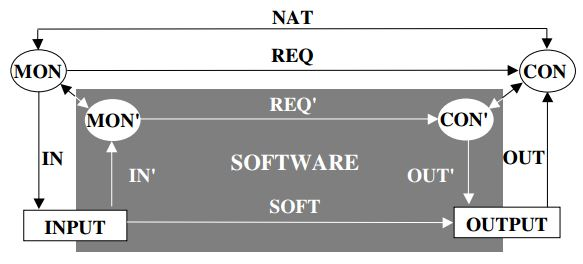
\includegraphics[scale=0.6] {images/FourVarExtn.jpg}
    \caption{Extension of Four Variable Model}
    \label{fig:extn-four-var}
 \end{figure}

To address this concern for the software, Miller et al extended the four variable model, as shown in Figure~\ref{fig:extn-four-var}. They recreate virtual versions of the variables $mon'$ and $con'$ that differ from the original $mon$ and $con$ in terms of value and timing introduced when sensing and setting the input and output variables. Using these virtual variables, they ``stretch'' the $SOF$ (software) relationship into $IN'$, $REQ'$, and $OUT'$. The $IN'$ and $OUT'$ represents the specification of hardware drivers that were previously part of the $SOF$. With this change, they propose a mere recapture of each function in $REQ$ to $REQ'$ using corresponding variables. They assert that this makes the tracing of the requirements REQ to the software ($REQ'$) direct and straightforward. While this approach superficially seems indisputable and makes the task of decomposition simpler, in our experience, we found that this approach could result in inaccurately specified and verified component requirements.

The overall system requirements especially for complex control systems such as GPCA are typically captured in such a way to accommodate certain degree of inaccuracies and imperfections. For example, lets consider a system level requirement:

\begin{quotation}
\emph{``In basal mode, the system shall infuse the drug at a flow rate within $BasalFr$ $\pm t$\% tolerance''}
\end{quotation}

The tolerance (t) in this requirement was included to accommodate inaccuracies of the physical components that is going to be used in the GPCA. Mathematically, this requirement is a relation, since the flow rate (output) is allowed to have range of values. When we decomposed the GPCA into various components and tried to allocate requirements to the software (one of the components of GPCA), we were tempted to formalize requirements for verification such that it mirrors the system requirement but in terms of inputs and outputs of the software, such as:
\\\\
\footnotesize{\texttt{
(Mode = basal) $\Rightarrow$\\
\textcolor{white}{------}FlowRate $\leq$ (1 + t/100) $\ast$ (BasalFr) and \\
\textcolor{white}{------}FlowRate $\geq$ (1 - t/100) $\ast$ (BasalFr)\\
}}
\normalsize{}\\
While the above formulation appears to be correct and mirrors the system level requirement, the tolerance part was not intended to be allocated to the software. When we model checked this requirement it was successfully verified since the software indeed satisfied, but in an unintended fashion. In reality, the software's output is deterministic and there was no need for the tolerance, hence the consequent in the formalization was supposed to be \texttt{(FlowRate $=$ BasalFr)}. That is, mathematically the requirement of the software is a function as opposed to the system level requirement that is a relation. %In our opinion, failing to understand these differences in mathematical formulation leads to inaccurate understanding of formal verification.

While superficially this doesn't appear to be a problem, an indepth analysis revels that this leads to a situation in which we could prove the system level requirements with just the software requirements. The way we formalized the software requirement is not only an over approximation of the capabilities of the software but also masks the other component requirements. Unfortunately, this was not apparently visible until we started analysing how the software requirements realizes the system level requirements.
